\def\orbitGraphCoords{\coordinate (A) at (0,0);\coordinate (B) at (1,0);\coordinate (C) at (1,1);\coordinate (D) at (0,1);}

\newcommand{\orbitOne}{\begin{tikzpicture}[scale=0.25, line cap=round, line width=1pt]
		\begin{scope}[shift={(0,0)}]
			\orbitGraphCoords
			\filldraw (A) circle (1pt);
			\filldraw (B) circle (1pt);
			\filldraw (C) circle (1pt);
			\filldraw (D) circle (1pt);
		\end{scope}
\end{tikzpicture}}

\newcommand{\orbitTwo}{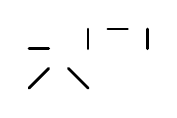
\begin{tikzpicture}[scale=0.25, line cap=round, line width=1pt]
		\begin{scope}[shift={(0,0)}]
			\orbitGraphCoords
			\draw (A)--(B);
		\end{scope}
		
		\begin{scope}[shift={(2,0)}]
			\orbitGraphCoords
			\draw (B)--(C);
		\end{scope}
		
		\begin{scope}[shift={(4,0)}]
			\orbitGraphCoords
			\draw (C)--(D);
		\end{scope}
		
		\begin{scope}[shift={(6,0)}]
			\orbitGraphCoords
			\draw (D)--(A);
		\end{scope}
		
		% one edge + one diagonal
		\begin{scope}[shift={(0,-2)}]
			\orbitGraphCoords
			\draw (A)--(C);
		\end{scope}
		
		\begin{scope}[shift={(2,-2)}]
			\orbitGraphCoords
			\draw (B)--(D);
		\end{scope}
\end{tikzpicture}}

\newcommand{\orbitThree}{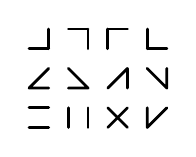
\begin{tikzpicture}[scale=0.25, line cap=round, line width=1pt]
		% adjacent edges
		\begin{scope}[shift={(0,0)}]
			\orbitGraphCoords
			\draw (A)--(B) (B)--(C);
		\end{scope}
		
		\begin{scope}[shift={(2,0)}]
			\orbitGraphCoords
			\draw (B)--(C) (C)--(D);
		\end{scope}
		
		\begin{scope}[shift={(4,0)}]
			\orbitGraphCoords
			\draw (C)--(D) (D)--(A);
		\end{scope}
		
		\begin{scope}[shift={(6,0)}]
			\orbitGraphCoords
			\draw (D)--(A) (A)--(B);
		\end{scope}
		
		% one edge + one diagonal
		\begin{scope}[shift={(0,-2)}]
			\orbitGraphCoords
			\draw (A)--(B) (A)--(C);
		\end{scope}
		
		\begin{scope}[shift={(2,-2)}]
			\orbitGraphCoords
			\draw (A)--(B) (B)--(D);
		\end{scope}
		
		\begin{scope}[shift={(4,-2)}]
			\orbitGraphCoords
			\draw (B)--(C) (A)--(C);
		\end{scope}
		
		\begin{scope}[shift={(6,-2)}]
			\orbitGraphCoords
			\draw (B)--(C) (B)--(D);
		\end{scope}
		
		% opposite edges
		\begin{scope}[shift={(0,-4)}]
			\orbitGraphCoords
			\draw (A)--(B) (C)--(D);
		\end{scope}
		
		\begin{scope}[shift={(2,-4)}]
			\orbitGraphCoords
			\draw (B)--(C) (D)--(A);
		\end{scope}
		
		% both diagonals / cross patterns
		\begin{scope}[shift={(4,-4)}]
			\orbitGraphCoords
			\draw (A)--(C) (B)--(D);
		\end{scope}
		
		\begin{scope}[shift={(6,-4)}]
			\orbitGraphCoords
			\draw (A)--(C) (A)--(D);
		\end{scope}
\end{tikzpicture}}

\newcommand{\orbitFour}{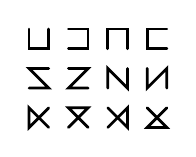
\begin{tikzpicture}[scale=0.25, line cap=round, line width=1pt]
		% cups
		\begin{scope}[shift={(0,0)}]
			\orbitGraphCoords
			\draw (D)--(A)--(B)--(C);
		\end{scope}
		
		\begin{scope}[shift={(2,0)}]
			\orbitGraphCoords
			\draw (A)--(B)--(C)--(D);
		\end{scope}
		
		\begin{scope}[shift={(4,0)}]
			\orbitGraphCoords
			\draw (B)--(C)--(D)--(A);
		\end{scope}
		
		\begin{scope}[shift={(6,0)}]
			\orbitGraphCoords
			\draw (C)--(D)--(A)--(B);
		\end{scope}
		
		% zigzags (row 2)
		\begin{scope}[shift={(0,-2)}]
			\orbitGraphCoords
			\draw (C)--(D)--(B)--(A);
		\end{scope}
		
		\begin{scope}[shift={(2,-2)}]
			\orbitGraphCoords
			\draw (D)--(C)--(A)--(B);
		\end{scope}
		
		\begin{scope}[shift={(4,-2)}]
			\orbitGraphCoords
			\draw (A)--(D)--(B)--(C);
		\end{scope}
		
		\begin{scope}[shift={(6,-2)}]
			\orbitGraphCoords
			\draw (D)--(A)--(C)--(B);
		\end{scope}
		
		% zigzags (row 3)
		\begin{scope}[shift={(0,-4)}]
			\orbitGraphCoords
			\draw (C)--(A)--(D)--(B);
		\end{scope}
		
		\begin{scope}[shift={(2,-4)}]
			\orbitGraphCoords
			\draw (A)--(C)--(D)--(B);
		\end{scope}
		
		\begin{scope}[shift={(4,-4)}]
			\orbitGraphCoords
			\draw (D)--(B)--(C)--(A);
		\end{scope}
		
		\begin{scope}[shift={(6,-4)}]
			\orbitGraphCoords
			\draw (D)--(B)--(A)--(C);
		\end{scope}
\end{tikzpicture}}

\newcommand{\orbitFive}{
\begin{tikzpicture}[scale=0.25, line cap=round, line width=1pt]
		\begin{scope}[shift={(0,0)}]
			\orbitGraphCoords
			\draw (A)--(B) (A)--(C) (A)--(D) (B)--(C) (B)--(D) (C)--(D);
		\end{scope}
\end{tikzpicture}}